\documentclass[12pt,a4paper]{article}

% Packages
\usepackage[utf8]{inputenc}
\usepackage{amsmath,amssymb}
\usepackage{graphicx}
\usepackage{geometry}
\usepackage{listings}
\usepackage{hyperref}

% Page Layout
\geometry{margin=1in}
\setlength{\parindent}{1cm}

% Code Listing Style
\lstset{basicstyle=\ttfamily, frame=single, breaklines=true, captionpos=b}

% Title Page Info
\title{Real Time Signal Processing for Proximity Sensor Data}
\author{Group 04: Uğur ÖZKAN(21050161003), Name2, Name3, Name4, Name5}
\date{\today}

\begin{document}

\maketitle
\section{Abstract}

The project aims to develop a dataset for obstacle detection and avoidance in autonomous drones, focusing on the challenging "focus of expansion" where optic flow is minimal. Data was collected using a drone equipped with multiple sensors, including event-based cameras, RGB cameras, radar, and IMU, with ground truth provided by an OptiTrack motion capture system. Experiments were conducted under varying light conditions and with different numbers of obstacles. The dataset comprises 1369 trials and is made available in ROS bag and CSV formats for research in navigation and obstacle avoidance.

\section{Introduction}

The primary challenge addressed is the difficulty autonomous drones face in reliably detecting and avoiding obstacles, especially in dynamic environments with changing lighting. Reliable obstacle detection is crucial for applications like drone delivery, search-and-rescue operations, and autonomous inspections. By addressing these challenges, the dataset promotes innovation in navigation algorithms and machine learning models for real-world scenarios.

\section{Methodology}
\textbf{Explain the methods and algorithms used, including relevant equations like:}
\begin{equation}
    y = mx + b
\end{equation}

Key algorithms process sensor data to extract features and insights, such as Fast Fourier Transform (FFT) applied to radar data to analyze signal magnitude and phase. Relevant equations include the FFT formula:
\begin{equation}
X(k) = \sum_{n=0}^{N-1} x(n) e^{-j\frac{2\pi k n}{N}}
\end{equation} 

This approach highlights periodic patterns crucial for radar-based obstacle detection.
\section{Data and Implementation}
\textbf{Briefly describe the dataset, preprocessing steps, and Python implementation. Include a code snippet if relevant:}

The dataset contains data from various sensors stored in CSV format. Preprocessing includes filtering noise and normalizing time series. For example, radar data undergoes FFT for frequency domain analysis, while IMU data uses sliding window filters for smoothing.

\begin{lstlisting}[language=Python, caption=Radar Data undergoes FFT]
import numpy as np
from scipy.fft import fft, fftshift

def fft_radar(re, im):
    s1 = fftshift(fft(re))
    s2 = fftshift(fft(im))
    magnitude = np.sqrt(s1.real**2 + s2.imag**2)
    return magnitude

# Load radar sample
radar_data = np.loadtxt('sample_radar.csv', delimiter=',')
real_part = radar_data[:, 1]
imag_part = radar_data[:, 2]
magnitude = fft_radar(real_part, imag_part)

\end{lstlisting}
\section{Results and Discussion}
\textbf{Present findings with graphs or screenshots:}

Using the provided scripts, radar data visualization showcases signal magnitude and phase for obstacle detection. IMU data plots reveal smoothed accelerations and angular velocities, supporting movement dynamics analysis. Below is an example visualization of FFT magnitude for radar data and smoothed IMU signals:

Graphs:

Radar FFT magnitude plot: Peaks indicate obstacle presence at specific distances.
IMU filtered accelerations: Smooth curves represent stability and noise reduction.
\begin{figure}[h!]
    \centering
    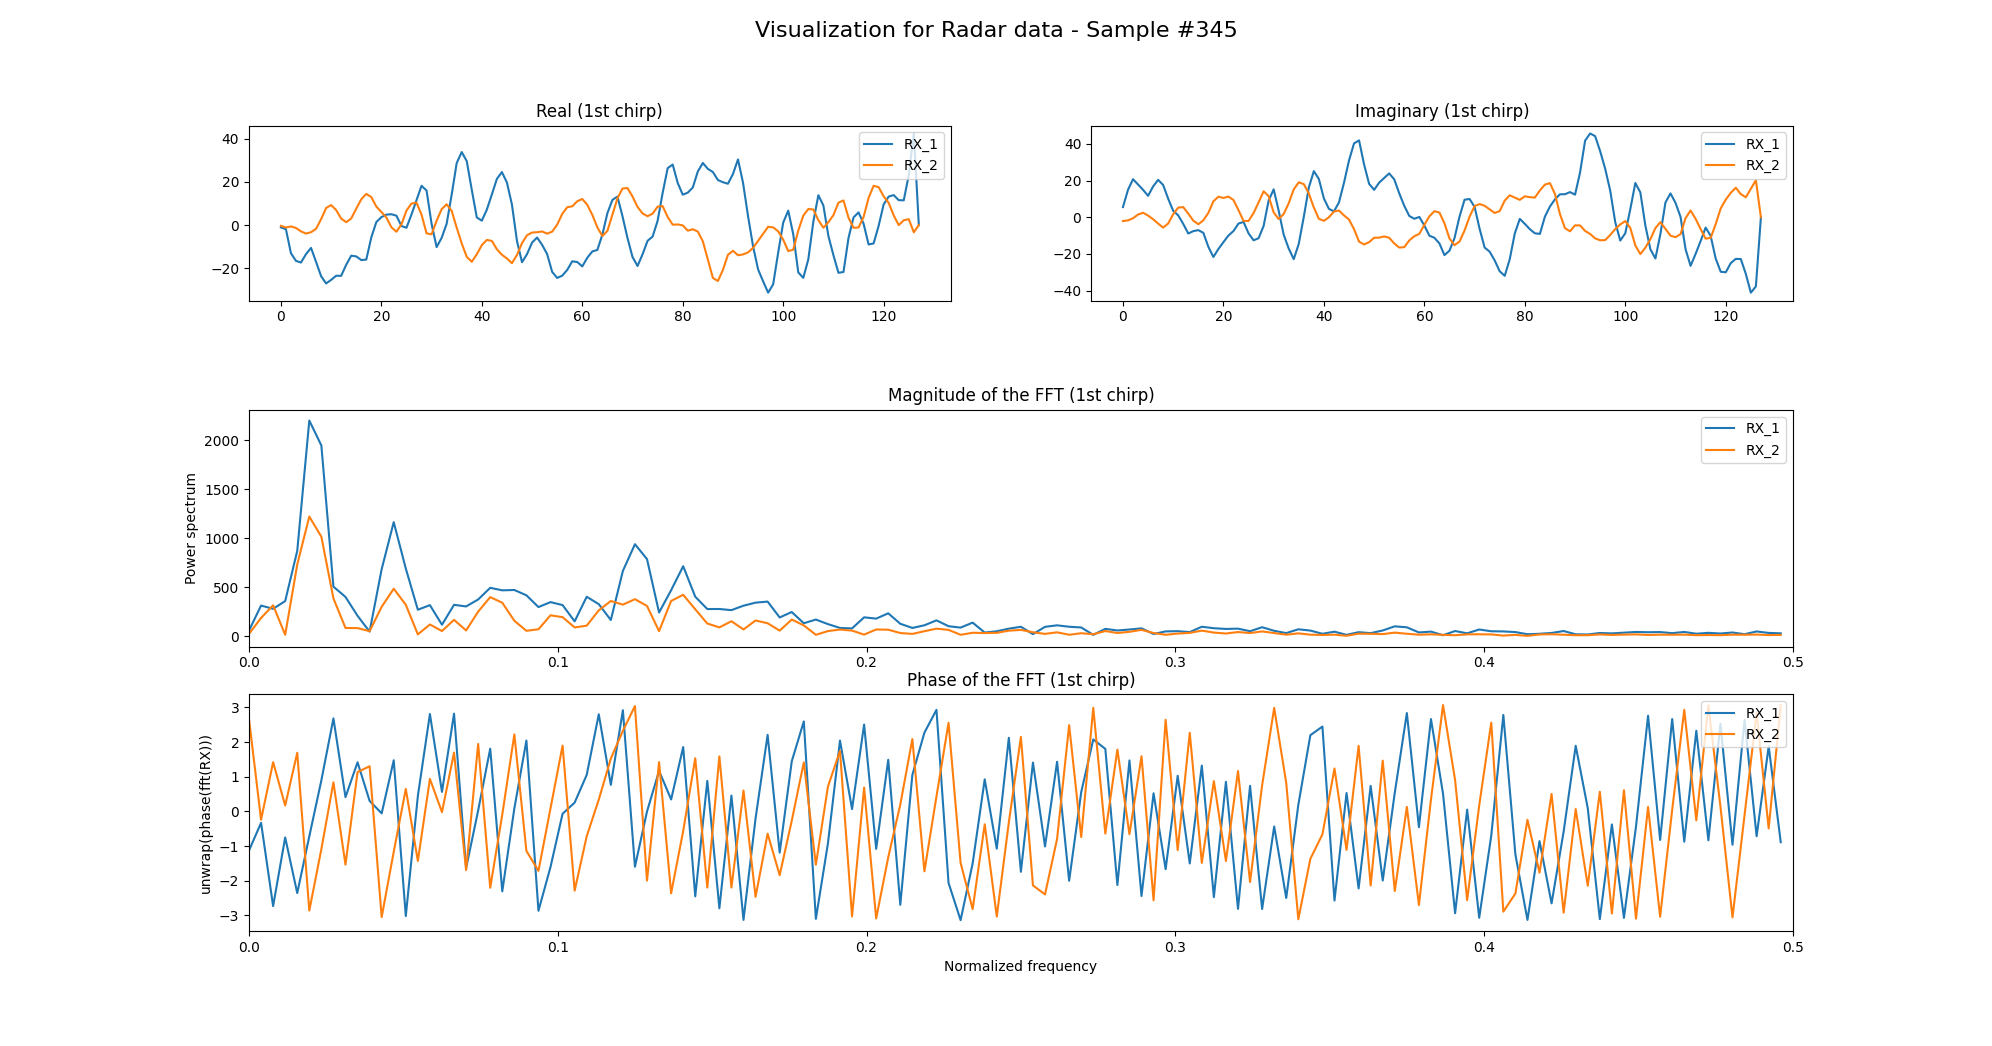
\includegraphics[width=0.8\textwidth]{radar_sample_345.png} 
    \caption{This is the graph of radar sample 345.}
    \label{fig:Radar_sample_345}
\end{figure}

\section{Conclusion}
\textbf{Summarize key outcomes and suggest future improvements.}

\section*{References}
\textbf{List all references, e.g., datasets, websites, or papers.}

\url{https://github.com/JuSquare/ODA_Dataset/tree/master}

\end{document}

